
\chapter{初期グラフによる探索空間の削減}
\label{chap:reduce-by-initial-graph}
\ref{sect:apply-to-gmg}節で述べた初期グラフを変更することで,
探索空間を削減できる.本章では,いくつかの初期グラフを与え,その効果を
実験により検証する.

\section{長さ$2Q+2$の閉路をもつ初期グラフ}
\label{sect:initial-graph-cycle}
長さ$2Q+2$の閉路を持つ初期グラフ$G_I$を次の手順で構築する.
ただし,$R(n,k)>0$を満たす$n,k$とする.
\begin{enumerate}
\item \ref{sect:apply-to-gmg}節で示した初期グラフを構築し,$G'_I$とする.
\item 次の3つの頂点$p,q,r$に対して,$G_I=G'_I\cup\{(p,r),(q,r)\}$とする.
  \begin{itemize}
  \item $p=n_{k,\hat{Q}-2}+1$
  \item $q=n_{k,\hat{Q}-2}+1+(k-1)^{\hat{Q}-2}$
  \item $r=n-R+1$
  \end{itemize}
\end{enumerate}

\begin{example}
  \label{ex:initial-graph-cycle}
  前述の手順に従って構築した,頂点数12,次数3の初期グラフを
  図\ref{fig:initial-graph-cycle-example}に示す.
  \begin{figure}
    \centering
    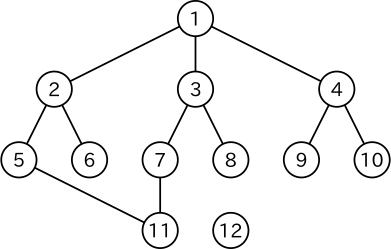
\includegraphics[width=.5\linewidth]{initial-tree-cycle-example.pdf}
    \caption{長さ6の閉路を含む,頂点数12,次数3の初期グラフ}
    \label{fig:initial-graph-cycle-example}
  \end{figure}
\end{example}

長さ$2Q+2$を含むグラフを初期グラフとすることの妥当性はまだ証明されていない.
(すでに証明されているかもしれない)
\begin{conjecture}
  一般化ムーアグラフ$M(n,k)$には,長さ$2Q+2$の閉路が少なくとも一つ存在する.
  ただし,$n>k+1$かつ,$R(n,k)>0$とする.
\end{conjecture}

\subsection*{候補辺の並べ替え}
長さ$2Q+2$の閉路を含む初期グラフから得られる候補辺は,頂点$v$に対する
$i_{<v}$と$i_{v>}$の値が大きくなるため,正則グラフであることの判定が遅くなり
探索が効率よく行えない.そこで,グラフの候補辺を次の手順で並べ替える.
並べ替え前の候補辺を$E$,並べ替え後の候補辺を$E'$とする.
\begin{enumerate}
\item 各頂点$v$について,$E$での出現回数を求める.これを$n_v$とする.
\item $w=\argmin_{v}(n_v)$の頂点$w$に対して,
  \begin{enumerate}
  \item $E'$の末尾に$E$中の$v$と接する辺集合を挿入する.
  \item 挿入した内容を$E$から削除する.
  \end{enumerate}
\item 上記を$E$が空になるまで繰り返す.
\end{enumerate}

\section{全域木}
\label{sect:initial-spanning-tree}
初期グラフとしての全域木を与える.次の手順で構築する.
\begin{enumerate}
\item 頂点$v\in\{2,\ldots,k+1\}$と頂点$1$とを隣接させる.
\item 頂点$v\in\{k+2,\ldots,n\}$に対して,次の式で求められる頂点$w$と
  隣接させる.
  \[ w=(v-n_{k,\hat{Q}(v)-1}-1)\mod(k(k-1)^{\hat{Q}(v)-2})+1+n_{k,\hat{Q}-1} \]
\end{enumerate}
このような全域木から探索することの妥当性は証明されていない.
\begin{conjecture}
  \label{conj:spanning-tree}
  一般化ムーアグラフ$M(n,k)$の全域木に,次の手順で構築した木が存在する.
  \begin{enumerate}
  \item 頂点$v\in\{2,\ldots,k+1\}$と頂点$1$とを隣接させる.
  \item 頂点$v\in\{k+2,\ldots,n\}$に対して,次の式で求められる頂点$w$と
    隣接させる.
    \[w=(v-n_{k,\hat{Q}(v)-1}-1)\mod(k(k-1)^{\hat{Q}(v)-2})+1+n_{k,\hat{Q}-1}\]
  \end{enumerate}
\end{conjecture}

また,条件を緩めて次のことも予想される.
\begin{conjecture}
  \label{conj:spanning-tree-2}
  一般化ムーアグラフ$M(n,k)$の全域木に,次の性質を満たす木が存在する.
  \begin{itemize}
  \item ある頂点からの距離が$Q$である頂点集合$V$について,
    $\max(d(v)\,|\,v\in V)-\min(d(v)\,|\,v\in V)\leq 1$
  \end{itemize}
\end{conjecture}

\begin{example}
  先に述べた手順に従っていくつかの全域木を構築する.
  構築した初期グラフを図\ref{fig:initial-spanning-tree-example}に示す.
  \begin{figure}
    \centering
    \subfloat[頂点数$12$,次数$3$の全域木]{
      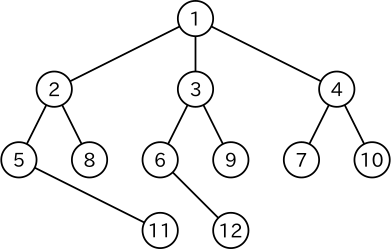
\includegraphics[width=.4\linewidth]
                      {initial-spanning-tree-12-example.pdf}
    }\hfill
    \subfloat[頂点数$18$,次数$3$の全域木]{
      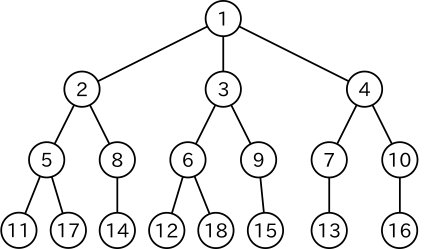
\includegraphics[width=.45\linewidth]
                      {initial-spanning-tree-18-example.pdf}
    }
    \caption{全域木の例}
    \label{fig:initial-spanning-tree-example}
  \end{figure}
\end{example}

\section{実験}
\label{sect:exp-reduce-by-initial}
アルゴリズム\ref{algo:basic-graph-initr}を先述した構築法で
置き換えるだけでよい.

\section{結果}
\label{sect:result-reduce-by-initial}
次数が3のときの実験結果を示す.
探索開始から最初の一般化ムーアグラフの発見における探索時間と状態の
取り出し回数を図\ref{fig:ginitr-time}と図\ref{fig:ginitr-node}に
それぞれ示す.また,一般化ムーアグラフの列挙におけるグラフ数と列挙時間と
状態の取り出し回数を図\ref{fig:ginitr-full-graph}と図\ref{fig:ginitr-full-time}と
図\ref{fig:ginitr-full-node}にそれぞれ示す.結果から,次のことが考察される.
指数関数的に増える(適当).

\begin{figure}
  \centering
  \includegraphics{the-ginitr-time.pdf}
  \caption{最初の一般化ムーアグラフの発見までの時間}
  \label{fig:ginitr-time}
\end{figure}
\begin{figure}
  \centering
  \includegraphics{the-ginitr-node.pdf}
  \caption{最初の一般化ムーアグラフの発見までの展開状態数}
  \label{fig:ginitr-node}
\end{figure}

\begin{figure}
  \centering
  \includegraphics{the-ginitr-full-graph.pdf}
  \caption{列挙された一般化ムーアグラフの数}
  \label{fig:ginitr-full-graph}
\end{figure}
\begin{figure}
  \centering
  \includegraphics{the-ginitr-full-time.pdf}
  \caption{一般化ムーアグラフの列挙に要した時間}
  \label{fig:ginitr-full-time}
\end{figure}
\begin{figure}
  \centering
  \includegraphics{the-ginitr-full-node.pdf}
  \caption{一般化ムーアグラフの列挙における展開状態数}
  \label{fig:ginitr-full-node}
\end{figure}
